\documentclass{rntz}
% Options: charter, cochineal, palatino, libertine
\usepackage[charter]{rntzfont}
%\usepackage[a5,width=115mm]{rntzgeometry}
%\usepackage[b5,width=350pt]{rntzgeometry}
\usepackage[b5,width=13cm]{rntzgeometry}
%\usepackage[a4]{rntzgeometry}

%% \documentclass{article}
%% \usepackage[b5paper]{geometry}
%% \usepackage[dvipsnames]{xcolor}
%% \definecolor[named]{ACMBlue}{cmyk}{1,0.1,0,0.1}
%% \definecolor[named]{ACMYellow}{cmyk}{0,0.16,1,0}
%% \definecolor[named]{ACMOrange}{cmyk}{0,0.42,1,0.01}
%% \definecolor[named]{ACMRed}{cmyk}{0,0.90,0.86,0}
%% \definecolor[named]{ACMLightBlue}{cmyk}{0.49,0.01,0,0}
%% \definecolor[named]{ACMGreen}{cmyk}{0.20,0,1,0.19}
%% \definecolor[named]{ACMPurple}{cmyk}{0.55,1,0,0.15}
%% \definecolor[named]{ACMDarkBlue}{cmyk}{1,0.58,0,0.21}
%% \usepackage{amsmath,amsthm}
%% \usepackage{hyperref,url,cleveref}
%% \theoremstyle{definition}
%% \newtheorem{theorem}{Theorem}
%% \newtheorem{conjecture}[theorem]{Conjecture}
%% \newtheorem{lemma}[theorem]{Lemma}
%% \theoremstyle{definition}
%% \newtheorem{definition}[theorem]{Definition}
%% \theoremstyle{remark}
%% \newtheorem*{corollary}{Corollary}
%% \theoremstyle{plain}            %back to default


%% ---- Packages ----
%\usepackage{adjustbox}          % aligning tikz diagrams vertically w/ tables.
\usepackage{amsmath,amssymb}    % basic math formatting & symbols
%\usepackage{anyfontsize}        % avoid font size warnings from stmaryrd
\usepackage{booktabs}           % \midrule
\usepackage{mathpartir}         % \mathpar, \infer
\usepackage{mathtools}          % for \dblcolon
\usepackage{multirow}           % \multirow, \multicolumn
\usepackage{stmaryrd}           % \llbracket, \rrbracket, \oast
\usepackage{tikz,tikz-cd}       % Hasse & commutative diagrams.

% typographic improvements
% TODO: put these in rntzfont.sty or rntz.cls?
\usepackage[spacing=true,stretch=15,tracking=true,letterspace=15]{microtype}
\frenchspacing


%% ---- Commands ----
\newcommand{\todo}[1]{{\color{Purple}#1}}

\newcommand{\fapremise}[1]{(\forall #1)~\,}

\newcommand{\bnfeq}{\dblcolon=}
%% \newcommand{\defeq}{\overset{\ms{def}}{=}}

\newcommand{\ms}[1]{\ensuremath{\mathsf{#1}}}
\newcommand{\mb}[1]{\ensuremath{\mathbf{#1}}}
\newcommand{\mi}[1]{\ensuremath{\mathit{#1}}}
\newcommand{\mc}[1]{\ensuremath{\mathcal{#1}}}

\newcommand{\GG}{\Gamma}
\newcommand{\N}{\mathbb{N}}
\newcommand{\x}{\times}
\newcommand{\fn}{\lambda}
\newcommand{\binder}{.~}
\newcommand{\bind}[1]{{#1}\binder}
\newcommand{\fnof}[1]{\fn\bind{#1}}
\newcommand{\sub}[1]{\{{#1}\}}
\newcommand{\fix}{\ms{fix}}
\newcommand{\den}[1]{\llbracket{#1}\rrbracket}

%% Category & preorder theory
\newcommand{\cat}[1]{\textsc{#1}} %category name
\newcommand{\Pre}{\cat{preord}}
\newcommand{\Set}{\cat{set}}
\newcommand{\Tone}{\cat{tone}}
\newcommand{\Cat}{\cat{cat}}

\newcommand{\idfn}{\mi{id}}
\newcommand{\isoto}{\simeq}
\newcommand{\pathto}{\sim}

%% Tone functors.
\newcommand{\id}{\ms{id}}
\newcommand{\op}{\ms{op}}
\newcommand{\iso}{\ms{iso}}     % iso, core, inv, eq
\renewcommand{\path}{\ms{path}} % path, loc, biv, bi
% Sensible combinations:
% {bi, eq}: suggestive, short.
%           DISLIKE: "bi" ambiguous. "eq" suggests equality.
% {inv, biv}: invariant, bivariant. DISLIKE: functor meaning nonobvious.
% {iso, path}: suggestive of generalization to categories
% {core, loc}: established-ish category theory notation. DISLIKE: opaque.

\newcommand{\tc}{\cdot}                      % tone composition
\newcommand{\tm}{\id}                        % monotone / id
\newcommand{\ta}{{\color{ForestGreen}\op}}   % antitone / op
\newcommand{\ti}{{\color{NavyBlue}\iso}}     % invariant/ core
\newcommand{\tb}{{\color{Bittersweet}\path}} % bivariant/ path


%% ---- Front matter ----
\title{Tones and Types}
\author{Michael Arntzenius, %
  \href{mailto:daekharel@gmail.com}{daekharel@gmail.com}}
% Date format: "25 March 2018"
\usepackage[en-GB]{datetime2}
\DTMlangsetup[en-GB]{ord=omit}
\date{\today}


\begin{document}

\maketitle

\begin{abstract}
 Certain properties of maps between preorders (e.g.\ preserving equivalence)
 reduce to monotonicity with respect to an altered domain ordering. I dub such
 alterations ``tones'', and explore their theory. I sketch a typed
 $\lambda$-calculus of monotone functions, using tones to allow selective
 non-mono\-tonicity.
\end{abstract}

\section{Preorders}

A preorder is a relation $a \le b$ satisfying:
\begin{enumerate}
\item \textbf{Reflexivity:} $a \le a$.
\item \textbf{Transitivity:} If $a \le b$ and $b \le c$ then $a \le c$.
\end{enumerate}

Preorders generalize partial orders by not requiring antisymmetry. Let $a \equiv
b$ iff $a \le b$ and $b \le a$. Antisymmetry means $a \equiv b$ implies $a = b$.
%
A good example preorder is ``lists under containment'', where $a \le b$ iff
every element of $a$ is also in $b$. Note that $[0,1] \equiv [1,0]$, but $[0,1]
\ne [1,0]$.

To a category theorist, a preorder is a ``thin'' category: between any two
objects there is at most one morphism. I suspect much of the ``tone theory'' in
this document, ostensibly about maps between preorders, extends to functors
between categories.


\section{Tones}\label{sec:tones}

Tones are ways a function $f$ may respect a preorder. I will consider four
tones, \tm, \ta, \ti, and \tb:

\begin{center}
  \begin{tabular}{clc@{\hskip 0.25em}c@{\hskip 0.25em}c}
    \multicolumn{1}{c}{\textit{Tone}}
    & \multicolumn{1}{c}{\textit{Name}}
    %% & \multicolumn{1}{c}{\textbf{Respects}}
    & \multicolumn{3}{c}{\textit{Property of $f$}}
    \\\midrule
    \tm & \text{Monotone}
    %% & \text{ordering}
    & $x \le y$ &$\implies$& $f(x) \le f(y)$
    \\
    \ta & \text{Antitone}
    %% & \text{opposite ordering}
    & $x \ge y$ &$\implies$& $f(x) \le f(y)$
    \\
    \ti & \text{Invariant}
    %% & \text{induced equivalence or ``isomorphisms''}
    & $x \le y \wedge y \le x$ &$\implies$& $f(x) \le f(y)$
    \\
    \tb & \text{Bivariant}
    %% & \text{equivalence closure or ``paths''}
    & $x \le y \vee y \le x$ &$\implies$& $f(x) \le f(y)$
  \end{tabular}
\end{center}

Informally,
\begin{enumerate}
\item $\tm$ is monotone (order-preserving).
\item $\ta$ is antitone (order-inverting).
\item $\ti$ is invariant, preserving only equivalence.
\item $\tb$ is bivariant: both monotone and antitone.
\end{enumerate}

%% In posets, antisymmetry trivializes invariance (because $x \le y \wedge y \le x
%% \implies x = y \implies f(x) = f(y)$), so we sometimes call $\ti$ the
%% ``discrete'' tone, because it respects only the discrete ordering.


\subsection{Tones transform orders}

Fix preorders $A, B$. Let $A^\op$ be $A$, ordered oppositely. Now, observe
that
%
\begin{center}
  $f : A \to B$ is antitone

  \nopagebreak \emph{iff} \nopagebreak

  $f : A^\op \to B$ is monotone
\end{center}

So ``antitone'' is a special case of ``monotone''! This observation generalizes:
every tone is really monotonicity with a transformation applied to the domain's
ordering. So \textbf{tones transform orders}. I write $A^s$ for the preorder $A$
transformed by the tone $s$, defined:

\begin{center}
  \begin{tabular}{clc@{\hskip 0.25em}c@{\hskip 0.25em}ll}
    {\textit{Tone}}
    & {\textit{Meaning}}
    & \multicolumn{3}{c}{\textit{Transformation on $A$}}
    \\\midrule
    \tm & \text{same ordering}
    & $a \le b : A$ &$\iff$& $a \le b : A^\tm$
    \\
    \ta
    & \text{opposite ordering}
    & $a \ge b : A$ &$\iff$& $a \le b : A^\op$
    \\
    \ti
    & \text{induced equivalence}
    & $a \le b \wedge b \le a : A$ &$\iff$& $a \le b : A^\iso$
    \\
    \tb{}
    & \text{equivalence closure}
    & $a \le b \vee b \le a : A$ &$\ \implies$& $a \le b : A^\path$
    %% & {\small\itshape see \ref{sec:defining-path}}
  \end{tabular}
\end{center}

With this, we can state the theorem generalizing our observation:
\begin{theorem}[Tones transform orders]\label{thm:tones-transform-orders}%
  %% For any function $f : A \to B$ between preorders $A$, $B$:
  ~\nopagebreak
  \begin{center}
    $f : A \to B$ has tone $s$

    \nopagebreak\emph{iff}\nopagebreak

    $f : A^s \to B$ is monotone
  \end{center}
\end{theorem}

From this point on, when I write $f : A \to B$, I mean implicitly that $f$ is
monotone; and therefore $f : A^s \to B$ means that $f$ has tone $s$.

Here are a few more useful properties of tones, which I invite you to verify:

\begin{theorem}[Functoriality of tones]\label{thm:tone-functoriality}
  If $f : A \to B$ then $f : A^s \to B^s$.
  %% \[\text{If}~ f : A \to B ~\text{then}~ f : A^s \to B^s\text{.}\]
\end{theorem}

\begin{theorem}[Tones distribute over $\x$ and $+$]\label{thm:tones-monoidal}
  \begin{eqnarray*}
    (A + B)^s = A^s + B^s\\
    (A \x B)^s = A^s \x B^s
  \end{eqnarray*}
\end{theorem}

\subsection{Understanding \iso{} and \path{}}

\todo{An intuition about $\ti$ and $\tb$: $\ti$ keeps only the \emph{strongly
    connected components}, while $\tb$ turns \emph{weakly} connected components
  into \emph{strong} ones. I should use an example, with diagrams. I should also
  mention that \iso{} and \path{} turn preorders into equivalence relations, and
  the corresponding cate\-gory-and-functor diagram.}

\subsection{Defining \path{}} \label{sec:defining-path}

$A^\path$ is the smallest preorder satisfying
\[ a \le b \vee b \le a : A \implies a \le b : A^\path \]

Unfortunately $A^\path$ is not so easy to define directly (without
language like ``the smallest preorder satisfying'')
%
because the reverse implication, from $a \le b : A^\path$ to $a \le b \vee b \le
a : A$, does not always hold. A good counterexample is the \ms{fencepost}
preorder on $\N$, where $a < a+1$ for even $a$, and $a > a+1$ for odd $a$:

\begin{center}
  \begin{tikzpicture}
    \node (0)    at ( 0, 0) {0};
    \node (1)    at ( 1, 1) {1};
    \node (2)    at ( 2, 0) {2};
    \node (3)    at ( 3, 1) {3};
    \node (4)    at ( 4, 0) {4};
    \node (5)    at ( 5, 1) {5};
    \node (6)    at ( 6, 0) {6};
    \node (dots) at ( 7, 1) {$\quad\cdots$};
    \draw (0) -- (1) -- (2) -- (3) -- (4) -- (5) -- (6) -- (dots);
  \end{tikzpicture}
\end{center}

Note that $a \le b \vee b \le a : \ms{fencepost} \iff |a-b| \le 1$, which isn't
transitive! Instead, $\ms{fencepost}^\path$ is the \emph{transitive closure} of
$|a-b| \le 1$, which makes everything equivalent:
\[ 0 \equiv 1 \equiv 2 \equiv 3 \equiv 4 \equiv \dots \]

This suggests a direct definition: let a \emph{path} from $a_0$ to $a_n$ be a
``zig-zag\-ging'' list $a_0, \dots, a_n$ such that $a_i \le a_{i+1} \vee a_i \ge
a_{i+1} : A$. Then $a \le b : A^\path$ iff there is a path from $a$ to $b$.


\subsection{Tone operators}

\begin{figure*}[t]
  \begin{mathpar}
    %% "baseline=(current bounding box.center)" incantation taken from
    %% https://tex.stackexchange.com/questions/220531/how-to-align-tikzpicture-and-text-in-a-table/220543#220543
    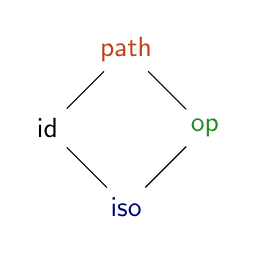
\begin{tikzpicture}[scale=1,baseline=(current bounding box.center)]
      \node (top)  at ( 0, 1) {$\tb$};
      \node (bot)  at ( 0,-1) {$\ti$};
      \node (-1)   at (-1, 0) {$\tm$};
      \node (1)    at ( 1, 0) {$\ta$};
      \draw (top) -- (-1) -- (bot) -- (1) -- (top);
    \end{tikzpicture}

    \begin{array}{r|cccc}
      s \wedge t
      & \tm & \tb & \ta & \ti\\\hline
      \tm & \tm & \tm & \ti & \ti\\
      \tb & \tm & \tb & \ta & \ti\\
      \ta & \ti & \ta & \ta & \ti\\
      \ti & \ti & \ti & \ti & \ti
    \end{array}

    \begin{array}{cr|cccc}
      \multicolumn{2}{c|}{\multirow{2}{*}{$s \tc t$}}
      & \multicolumn{4}{c}{t}\\
      && \tm & \ta & \ti & \tb\\\hline
      \multirow{4}{*}{$s$}
      & \tm & \tm & \ta & \ti & \tb\\
      & \ta & \ta & \tm & \ti & \tb\\
      & \ti & \ti & \ti & \ti & \ti\\
      & \tb & \tb & \tb & \tb & \tb
    \end{array}
  \end{mathpar}
  \caption{Tone lattice, meet, and composition}
  \label{fig:tone-ops}
\end{figure*}

\Cref{fig:tone-ops} defines two operators on tones:
\begin{enumerate}
\item Meet $s \wedge t$ is greatest lower bound in the lattice ordered $\ti
  < \{\tm, \ta\} < \tb$. This gives the general tone of the pairing $\langle f,
  g\rangle : A^{s \wedge t} \to B \times C$ of two functions $f : A^s \to B$ and
  $g : A^{t} \to C$.

\item Composition $s \tc t$ gives the tone of a composed function $g \circ f :
  A^{s \tc t} \to C$ when $f : A^s \to B$ and $g : B^t \to C$. Equivalently,
  $A^{s\tc t} = (A^s)^t$ for any preorder $A$.
\end{enumerate}

Together, $\wedge$ and $\tc$ form a semiring whose properties are given in
\cref{fig:tone-op-laws}. \todo{TODO: Reference ``I Got Plenty o' Nuttin'{}'' ---
  another use of variable annotations drawn from a semiring, and with similar
  (the same?) behavior of those annotations in the inference rules.}

\todo{TODO: check the distribution laws hold!}

\begin{figure*}
  \begin{mathpar}
    \begin{array}{lr@{\hskip 0.5em}c@{\hskip 0.5em}l}
      \multicolumn{4}{c}{\textit{\normalsize Properties of ${}\wedge{}$}}
      \vspace{2pt}\\
      \text{Associativity} & (s \wedge t) \wedge u &=& s \wedge (t \wedge u)\\
      \text{Commutativity} & s \wedge t &=& t \wedge s\\
      \text{Idempotence} & s \wedge s &=& s\\
      \tb~\text{is identity} & \tb \wedge s &=& s\\
      \ti~\text{absorbs} & \ti \wedge s &=& \ti\\
    \end{array}

    \begin{array}{lr@{\hskip 0.5em}c@{\hskip 0.5em}l}
      \multicolumn{4}{c}{\textit{\normalsize Properties of ${}\tc{}$}}
      \vspace{2pt}\\
      \text{Associativity} & (s \tc t) \tc u &=& s \tc (t \tc u)\\
      \text{Identity} & \multicolumn{3}{c}{\tm \tc s = s = s \tc \tm}\\
      \tb~ \text{left-absorbs} & \tb \tc s &=& \tb\\
      \ti~ \text{left-absorbs} & \ti \tc s &=& \ti\\
      \ta~ \text{self-inverts} & \ta \tc \ta &=& \tm\\
    \end{array}

    \begin{array}{lr@{\hskip 0.5em}c@{\hskip 0.5em}l}
      \text{Left-distribution} & s \tc (t \wedge u) &=& (s \tc t) \wedge (s \tc u)\\
      \text{Right-distribution} & (s \wedge t) \tc u &=& (s \tc u) \wedge (t \tc u)
    \end{array}
  \end{mathpar}
  \caption{Properties of tone operators}
  \label{fig:tone-op-laws}
\end{figure*}

\subsection{Monotonicity Types}

\href{https://infoscience.epfl.ch/record/231867/files/monotonicity-types.pdf}{\emph{Monotonicity
    Types}} by Clancy, Miller, and Meiklejohn has similar tables for their
composition $\circ$ and ``contraction'' $+$ operators! However, instead of
bivariance they have constancy, a stricter condition.
%
Constancy corresponds to respecting the \emph{indiscrete ordering} (which sets
$a \le b$ for all $a,b$).\footnote{Indiscreteness and its dual, discreteness,
  are also tones --- that is, functorial transformations on the ordering
  component of a preorder --- but they complicate things, so I omit them.

  Note also that discreteness and $\ti$ coincide on posets; many intuitions
  transfer from one to the other.}
%
Interestingly, because constancy is so much stricter than bivariance, their
composition operator is commutative.

They write $\uparrow$ for $\tm$, $\downarrow$ for $\ta$, $?$ for $\ti$, and
$\sim$ for constancy. They also add $=$ for the ``tone'' that \emph{only the
  identity function} has. This doesn't fit my framework; it cannot be phrased as
a transformation on orderings. However, it seems related to subtyping.



\section{Tones, categorically}

\newcommand{\elemset}[1]{\ensuremath{|{#1}|}}
\newcommand{\elemsetfn}[0]{\elemset{-}}

This section gives a categorical semantics of tones. You may safely skip it.

Let's change perspective. \Cref{sec:tones} defines tones as function
pro\-per\-ties, then gives corresponding pre\-order trans\-form\-ations. Now,
let's define tones as preorder transformations, and derive corresponding
function properties.

\begin{definition}
  $\elemsetfn : \Pre \to \Set$ is the functor taking a preorder to its set of
  elements.
\end{definition}

\begin{definition}[Tones]\label{def:tone}
  A tone $s$ is a functor $-^s : \Pre \to \Pre$ such that $\elemset{-^s} =
  \elemsetfn$.\footnote{A more categorical approach might require only a natural
    isomorphism \(\iota : \elemset{-^s} \isoto \elemsetfn\). I'm not yet
    comfortable generalizing that far. }
\end{definition}

\begin{corollary}
  For any preorder $A$ and monotone map $f$,
  \begin{enumerate}
  \item $|A^s| = |A|$: tone functors alter a preorder's \emph{ordering}, not its
    elements.
  \item $|f^s| = |f|$: tone functors do not alter functions' behavior.
  \end{enumerate}
\end{corollary}

\begin{definition}
  A function $f$ from $A$ to $B$ has tone $s$ iff $f : A^s \to B$ is monotone.
\end{definition}

%% It's also unclear how to generalize this definition to tones of functors on
%% \Cat{}.

\subsection{Tone composition}

Tone composition $s \tc t$ corresponds to composition of tone functors:

\begin{theorem}
  The composition $(-^s)^t$ of two tones is itself a tone.
\end{theorem}

\begin{proof} Applying \cref{def:tone}, we have
  \( \elemset{(-^s)^t} = \elemset{-^s} = \elemsetfn \).
\end{proof}


\subsection{The \Tone{} category}

Preorders have a natural partial order, letting $A \le B$
iff $A$ is a \emph{subpreorder} of $B$ --- that is, if $\fnof{x} x : A \to
B$.\footnote{In other words, if $A \subseteq B$ and $x \le y : A \implies x \le
  y : B$.}
%
This lifts pointwise to a partial order on tones: let $s \le t$ iff $A^s \le
A^t$ for all $A$.
%
As functors, tones also form a category, \Tone{}, with natural transformations
as morphisms. However, \Tone{} is but a fa\c{c}ade over this partial order:

\begin{theorem} \label{thm:tone-poset}
  \[s \le t \iff \exists \eta : \Tone(s, t) \iff \exists! \eta : \Tone(s,t)\]
\end{theorem}

\begin{proof}
  Expanding definitions, $s \le t$ means $\fnof{x} x : A^s \to A^t$ for all $A :
  \Pre$. By \cref{lem:tone-transformations-are-id}, any $\eta : \Tone(s,t)$
  is of the form $\eta_A = \fnof{x} x : A^s \to A^t$.
\end{proof}

The crux here is that natural transformations between tones are \emph{boring}:
\begin{lemma}\label{lem:tone-transformations-are-id}
  For any natural transformation $\eta : -^s \to -^t$, we have $\eta_A = \fnof{x} x$.
\end{lemma}

\begin{proof}
  Let $\mb{1}$ be the singleton preorder $\{\star\}$. Fix some $x : A$. Let $f :
  \mb{1} \to A = \fnof{\star}{x}$. Then by naturality of $\eta$, this square
  commutes:
  %
  \[\tikzset{
    no line/.style={draw=none,
      commutative diagrams/every label/.append style={/tikz/auto=false}}}
  \begin{tikzcd}[sep=3.3em]
    \mb{1} \arrow[r,"\textstyle \eta_{\mb{1}}"] \arrow[d,"\textstyle f^s"]
    & \mb{1} \arrow[d,"\textstyle f^t"]
    \\ A^s \arrow[r,"\textstyle\eta_A"]
    & A^t
  \end{tikzcd}\]

From \cref{def:tone}, $f^s = f = f^t$; and since $\mb{1}$ is a singleton,
$\eta_{\mb{1}} = \idfn$, thus:
  \[\begin{array}{rlcl}
  & \eta_A \circ f^s &=& f^t \circ \eta_{\mb{1}}\\
  \implies & \eta_A \circ f &=& f\\
  \implies & \eta_A(x) &=& x
  \end{array}\]
\end{proof}

%% However, \Tone{} is a ``thin''
%% category: between two tones $s,t$ there is at most one natural transformation
%% $\eta : -^s \to -^t$.

%% \begin{definition}\label{def:tone-cat}
%%   \Tone{} is the category of tones and natural transformations between them.
%% \end{definition}


\subsection{The \Tone{} lattice}

\begin{conjecture}
  \Tone{} is a distributive lattice.
\end{conjecture}
\begin{proof}
  \todo{TODO}
\end{proof}

\todo{Isn't $\wedge$ greatest lower bound / product? Don't we have
  $\vee$ / least upper bound / coproducts? Old stuff:}

Tone meet $\wedge$ and composition $\tc$ also have semantic versions. $s \wedge
t$ corresponds to intersection of relations (noting that the intersection of two
reflexive, transitive relations is itself reflexive and transitive), and $s \tc
t$ corresponds to functor composition.
%
\begin{eqnarray*}
  a \le b : A^{s \wedge t} %% \iff a \le b : A^s \cap A^t
  &\iff& a \le b : A^s \wedge a \le b : A^t\\
  a \le b : A^{s \tc t} &\iff& a \le b : (A^s)^t
\end{eqnarray*}

\begin{conjecture}
  The intersection of two tones is a tone.
\end{conjecture}
\begin{proof}
  \todo{TODO}
\end{proof}

\begin{conjecture}
  The definitions of $\wedge$ and $\tc$ in \cref{fig:tone-ops} coincide with
  their semantic definitions, applied to the semantic interpretation of $\tm$,
  $\ta$, $\tb$, and $\ti$.
\end{conjecture}


\section{A tonal sequent calculus}

\begin{mathpar}
  (A_1^{t_1}, \dots, A_n^{t_n})^u = (A_1^{t_1 \tc u}, \dots, A_n^{t_n \tc u})\\

  \infer[Hypothesis]{t \le \tm}{\GG, A^t \vdash A}

  \infer[$T$-Right]{\GG \vdash A}{\GG^t \vdash T_t A}

  \infer[$T$-Left]{\GG{},A^{t\tc u} \vdash C}{\GG{}, (T_t A)^u \vdash C}

  \infer[Weakening]{\GG{}, A^t \vdash C \\ u \le t}{\GG{}, A^u \vdash C}

  \infer[Contraction]{\GG{},A^t, A^u \vdash C}{\GG{}, A^{t \wedge u} \vdash C}

  \infer[Cut]{\GG \vdash A \\ \Delta,A^t \vdash C}{\GG^t,\Delta \vdash C}
\end{mathpar}

Jason Reed sent me these rules for a sequent calculus with a connective $T_s$
internalizing the tone functor $-^s$. I aim to adapt this into a
natural-deduction-style system with proof terms, i.e.\! a simply typed
$\lambda$-calculus.


\section{A bidirectional \texorpdfstring{$\lambda$}{lambda}-calculus with tone inference}

\newcommand{\subtype}[3]{#2^{#1}\sqsubset {#3}}
\newcommand{\converts}[3]{#2^{#1} \prec {#3}}

\newcommand{\h}[3]{#1 : #2^{#3}} % hypotheses
\newcommand{\infers}[3]{{#1} \Rightarrow {#2} \vdash {#3}}
\newcommand{\checks}[3]{{#1} \Leftarrow {#2} \vdash {#3}}

%% \renewcommand{\infers}[3]{{#1} ~\shortrightarrow~ {#2} \vdash {#3}}
%% \renewcommand{\checks}[3]{{#1} ~::~ {#2} \vdash {#3}}

%% \renewcommand{\infers}[3]{{#2}\vdash {#1} \shortrightarrow {#3}}
%% \renewcommand{\checks}[3]{{#2}\vdash {#1} : {#3}}

\newcommand{\ein}{\ms{in}}
\newcommand{\einj}[2]{\ein_{#1}\:{#2}}
\newcommand{\einl}[1]{\einj{1}{#1}}
\newcommand{\einr}[1]{\einj{2}{#1}}
\newcommand{\cto}{\shortrightarrow}
\newcommand{\ecase}[5]{%
  \mb{case}~{#1}~\mb{of}\ {\einl{#2} \cto #3};\ {\einr{#4} \cto #5}}
\newcommand{\emptycx}{\cdot}

\begin{mathpar}
  \begin{array}{rccl}
    \text{variables} & x\\
    \text{base types} & P\vspace{0.5em}\\
    \text{tones} & s,t,u & \bnfeq & \tm ~|~ \ta ~|~ \tb ~|~ \ti
    \vspace{0.5em}\\
    \text{types} & A,B,C
    &\bnfeq& P ~|~ A \to B ~|~ A \x B ~|~ A + B ~|~ \Box A ~|~ \op\;A
    \vspace{0.5em}\\
    \text{checking terms} & m,n
    &\bnfeq& e ~|~ \fnof{x} m ~|~ (m,n) ~|~ \einj{i}{m}\\
    &&|& \mb{let}~x = e~\mb{in}~ m\\
    &&|& \ecase{e}{x}{m}{y}{n}
    \vspace{0.5em}\\
    \text{inferring terms} & e
    &\bnfeq& x ~|~ e\;m ~|~ \pi_i\;e ~|~ m : A
    \vspace{0.5em}\\
    \text{contexts}
    & \GG &\bnfeq& \emptycx ~|~ \GG{}, \h{x}{A}{s}
    \vspace{0.5em}\\
    \text{judgments}
    & J &\bnfeq&
    \checks{m}{\GG}{A} ~~|~~ \infers{e}{\GG}{A}\\
    &&|& \subtype{s}{A}{B} ~~|~~ \converts{s}{A}{B}
  \end{array}
\end{mathpar}

\todo{TODO: explain my various abuses of notation, e.g. $\GG^t$ and $\GG_1 \wedge
  \GG_2$}


\subsection{Typing rules}

%% \noindent\textbf{Inferring forms}
\subsubsection{Inferring forms}
%
\begin{mathpar}
  %% ---- inferring forms ----
  %% checking -> inferring by annotation
  \infer{\checks{m}{\GG}{A}}{\infers{m : A}{\GG}{A}}

  %% variables
  \infer{ }{\infers{x}{\h{x}{A}{\tm}}{A}}

  %% projection
  \infer{\infers{e}{\GG}{A} \\ \converts{s}{A}{B_1 \x B_2}}
        {\infers{\pi_i\;e}{\GG^s}{B_i}}

  %% application
  \infer{\infers{e}{\GG_1}{A}
         \\ \converts{u}{A}{B \to C}
         \\ \checks{m}{\GG_2}{B}}
        {\infers{e\; m}{\GG_1^u \wedge \GG_2}{C}}
\end{mathpar}

%% \noindent\textbf{Checking forms}
\subsubsection{Checking forms}
%
\begin{mathpar}
  %% ---- checking forms ----
  %% inferring -> checking by subtyping
  \infer{\infers{e}{\GG}{A} \\ \subtype{t}{A}{B}}
        {\checks{e}{\GG^t}{B}}

  %% automatic box and op introduction
  \infer{\checks{m}{\GG}{A}}
        {\checks{m}{\GG^\ti}{\Box A}}

  \infer{\checks{m}{\GG}{A}}
        {\checks{m}{\GG^\ta}{\op\; A}}

  %% let-binding
  \infer{\infers{e}{\GG_1}{A} \\ \checks{m}{\GG_2,\, \h{x}{A}{s}}{C}}
        {\checks{\mb{let}~x = e~\mb{in}~m}{\GG_1^s \wedge \GG_2}{C}}

  %% lambdas
  \infer{\checks{m}{\GG{},\, \h{x}{A}{s}}{B} \\ \tm \le s}
        {\checks{\fnof{x} m}{\GG}{A \to B}}

  %% pairs
  \infer{\checks{m}{\GG_1}{A_1} \\ \checks{n}{\GG_2}{A_2}}
        {\checks{(m,n)}{\GG_1 \wedge \GG_2}{A_1 \x A_2}}

  %% injection
  \infer{\checks{m}{\GG}{A_i}}
        {\checks{\einj{i}{m}}{\GG}{A_1 + A_2}}

  %% case analysis
  \infer{\infers{e}{\GG}{A} \\
         \converts{s}{A}{B_1 + B_2} \\
         \checks{m}{\GG_1,\, \h{x}{B_1}{t_1}}{C} \\
         \checks{n}{\GG_2,\, \h{y}{B_2}{t_2}}{C}}
        {\checks{\ecase{e}{x}{m}{y}{n}}
                {\GG^{s\tc(t_1\wedge t_2)} \wedge \GG_1 \wedge \GG_2}
                {C}}
\end{mathpar}


\subsection{Subtyping}

In $\subtype{s}{A}{B}$, the types $A$ and $B$ are inputs, and the tone $s$ is
output.
%
``$P~\text{equiv}$'' holds iff the base type $P$'s preorder is symmetric (i.e.\!
an equivalence relation).
%
\begin{mathpar}
  \infer{ }{\subtype{\tm}{A}{A}}

  \infer{P~\text{equiv}}{\subtype{\ti}{P}{P}}

  \infer{\subtype{s}{A}{B}}
        {\subtype{s \tc \ti}{A}{\Box B}}

  \infer{\subtype{s}{A}{B}}
        {\subtype{\tb \tc s}{\Box A}{B}}

  \infer{\subtype{s}{A}{B}}
        {\subtype{\ta \tc s}{(\op\; A)}{B}}

  \infer{\subtype{s}{A}{B}}
        {\subtype{s \tc \ta}{A}{\op\; B}}

  %% Products
  \infer{\subtype{s}{A_1}{A_2} \\ \subtype{t}{B_1}{B_2}}
        {\subtype{s \wedge t}{(A_1 \x B_1)}{A_2 \x B_2}}

  %% Sums
  \infer{\subtype{s}{A_1}{A_2} \\ \subtype{t}{B_1}{B_2}}
        {\subtype{s \wedge t}{(A_1 + B_1)}{A_2 + B_2}}
\end{mathpar}

Function subtyping, $\subtype{s}{(A_1 \to B_1)}{A_2 \to B_2}$, has four rules
--- one for each tone $s$ produced by $\subtype{s}{B_1}{B_2}$:
%
\begin{mathpar}
  \infer{\subtype{s}{A_1}{A_2} \\ \subtype{\tm}{B_1}{B_2} \\ \tm \le s}
        {\subtype{\tm}{(A_1 \to B_1)}{A_2 \to B_2}}

  \infer{\subtype{s}{A_1}{A_2} \\ \subtype{\ta}{B_1}{B_2} \\ \ta \le s}
        {\subtype{\ta}{(A_1 \to B_1)}{A_2 \to B_2}}

  \infer{\subtype{s}{A_1}{A_2} \\ \subtype{\tb}{B_1}{B_2} \\ \ti < s}
        {\subtype{\tb}{(A_1 \to B_1)}{A_2 \to B_2}}

  \infer{\subtype{\tb}{A_1}{A_2} \\ \subtype{\ti}{B_1}{B_2}}
        {\subtype{\ti}{(A_1 \to B_1)}{A_2 \to B_2}}
\end{mathpar}

\todo{Can these $t \le s$ constraints be turned into ``composing with $u$
  is $\ge \tm$'', for some choice of $u$ depending on $t$?}


\subsection{Modal stripping}

$\converts{s}{A}{B}$ is a specialization of $\subtype{s}{A}{B}$ which strips off
modal operators on $A$, turning them into transformations on $s$. As in
subtyping, $A$ is an input and $s$ an output; however, $B$ is now an output.
%
\begin{mathpar}
  \infer{A~\text{stripped}}{\converts{\tm}{A}{A}}

  \infer{\converts{s}{A}{B}}{\converts{\tb\tc s}{\Box A}{B}}

  \infer{\converts{s}{A}{B}}{\converts{\ta\tc s}{(\op\; A)}{B}}
\end{mathpar}

``$A~\text{stripped}$'' holds iff $A$ is \emph{not} of the form $\Box B$ or
$\op\; B$, i.e. its outermost connective is not modal.


\subsection{Tones and the \texorpdfstring{$\fn$}{lambda} rule}

Here are two more general variations on the $\fn$ rule I've considered:
%
\begin{mathpar}
  \infer[Fn-1]
        {\checks{m}{\GG{},\, \h{x}{A}{s}}{B} \\ A \sqsubset A^s}
        {\checks{\fnof{x}{m}}{\GG}{A \to B}}

  \infer[Fn-2]
        {\checks{m}{\GG{},\, \h{x}{A}{t}}{B}
         \\ \subtype{s}{A}{A}
         \\ \tm \le s \tc t}
        {\checks{\fnof{x} m}{\GG}{A \to B}}
\end{mathpar}
\textsc{Fn-1} requires a new judgment, $A \sqsubset B^s$, where $A,B,s$ are all
inputs; this doesn't seem difficult to define, but it's Yet Another Subtyping
Judgment. \textsc{Fn-2} avoids this, but is much less easy to explain.

However, it's not clear to me I need to generalize the $\fn$ rule. The reason I
thought I did was to justify something like the following:
\begin{mathpar}
  \infer*{\infer*{\vdots}
           {{\GG{},\, \h{x}{A}{\ti}} \vdash {m} : {B}}}
         {{\GG} \vdash {\fnof{x}{m}} : {\Box A \to B}}
\end{mathpar}

But this \emph{could} check as follows:
\begin{mathpar}
  \infer*{\infer*{\vdots}{\checks{m}{\GG{},\, \h{x}{\Box A}{s}}{B}}
          \\ \tm \le s}
         {\checks{\fnof{x}{m}}{\GG}{\Box A \to B}}
\end{mathpar}

So the crucial question is: can we always substitute $\h{x}{\Box A}{\tm}$ for
$\h{x}{A}{\ti}$?
%
It would suffice to prove the subtyping and substitution principles given in
\cref{sec:principles}. Can we prove these with our original, subtyping-less
$\lambda$ rule?


\section{Pattern matching}

\newcommand{\xbar}[2]{\overline{#2}^{#1}}
\newcommand{\pwild}{\_}
\newcommand{\pcheck}[3]{#1 : #2 \vdash #3}
\newcommand{\casecheck}[6]{%
  #1 \cto #2 \Leftarrow #3 \vdash {#4}^{#5} >\!\!> #6}
\renewcommand{\casecheck}[6]{%
  #1 \cto #2 \Leftarrow #3 \vdash {#4}^{#5} \rightsquigarrow #6}

\newcommand{\mdist}[2]{#1 \equiv #2}
\newcommand{\mbinop}{\boxplus}

\[\begin{array}{rccl}
  \text{patterns} & p,q
  &\bnfeq& x ~|~ (p,q) ~|~ \einj{i}{p}
  \vspace{0.5em}\\
  \text{checking terms} & m,n
  &\bnfeq& \mb{case}~ e ~\mb{of}~ \xbar{i}{p_i \cto m_i}
  \vspace{0.5em}\\
  \text{toneless contexts} & \phi,\psi &\bnfeq& \emptycx ~|~ \phi,\, x : A
  \vspace{0.5em}\\
  \text{distributive type ops} & \boxplus &\bnfeq& {\x} ~|~ {+}
  \vspace{0.5em}\\
  \text{judgments} & J
  &\bnfeq& \mdist{A}{B \mbinop C}\\
  &&|& \pcheck{p}{A}{\phi}\\
  &&|& \casecheck{p}{m}{\GG}{A}{s}{C}
\end{array}\]

\vspace{.5em} The types in toneless contexts $\phi$ aren't annotated with tones.
\todo{TODO: Explain why and when we use toneless contexts. Explain
  $\phi^{\vec{t}}$ notation for a context split into its types and its tones.}


\subsection{Distributing modes}

The pattern $(x,y)$ matches values of type $A \x B$. But how shall we match
values of type $\Box(A \x B)$?
%
We might add a pattern, $\mb{box}~p$, matching values of type $\Box A$. Then
$\mb{box}~(x,y)$ would match values of type $\Box(A \x B)$.
%
But do we \emph{need} this \mb{box} annotation? \Cref{thm:tones-monoidal} says
$\Box(A \x B)$ and $\Box A \x \Box B$ mean the same thing. Why not let $(x,y)$
match $\Box(A \x B)$ \emph{directly}, yielding $x : \Box A$ and $y : \Box B$?

To this end, we'll need a judgment $\mdist{A}{B \mbinop C}$ for distributing modes
over an operator $\mbinop$ (either $\x$ or $+$). Here $A$ is an input and
$B$, $C$ are outputs.
%
\begin{mathpar}
  \infer{ }{\mdist{A \mbinop B}{A \mbinop B}}

  \infer{\mdist{A}{B \mbinop C}}{\mdist{\Box A}{\Box B \mbinop \Box C}}

  \infer{\mdist{A}{B \mbinop C}}{\mdist{\op~ A}{\op\, B \mbinop \op~ C}}
\end{mathpar}


\subsection{Typing patterns}

The judgment $\pcheck{p}{A}{\phi}$ corresponds to a \Pre-morphism $A \to 1 +
\phi$. It means that the pattern $p$, when it matches a value of type $A$,
produces values for $\phi$'s variables.
%
\begin{mathpar}
  \infer{ }{\pcheck{x}{A}{x : A}}

  \infer{\mdist{A}{A_1 + A_2} \\ \pcheck{p}{A_i}{\phi}}
        {\pcheck{\einj{i}{p}}{A}{\phi}}

  \infer{\mdist{A}{A_1 \x A_2} \\
         \fapremise{i} \pcheck{p_i}{A_i}{\phi_i}\\
         \phi_1,\phi_2~\text{disjoint}}
        {\pcheck{(p_1, p_2)}{A}{\phi_1,\phi_2}}
\end{mathpar}

%% To handle non-linear patterns, or patterns with gu\-ard expressions, the
%% morphism would also need an input context $\GG$. I consider this in
%% \cref{sec:patterns-with-guards}.


\subsection{Typing \mb{case}-expressions}

Typing \mb{case} as a single rule is complicated:
%
\[
\infer{
  \infers{e}{\GG}{A} \\
  \fapremise{i} p_i : A \vdash \phi_i\\
  \fapremise{i} \checks{m_i}{\GG_i,\phi_i^{\vec{s}_i}}{C}
}{
  \checks{\mb{case}~e~\mb{of}~\xbar{i}{p_i \cto m_i}}
         {\GG^{\bigwedge_i\bigwedge\vec{s}_i} \wedge \bigwedge_i \GG_i}
         {A}}
\]
%% \begin{mathpar}
%%   \infer{\infers{e}{\GG}{A} \\
%%     (\forall i)~{\pcheck{p_i}{A}{s_i}{\phi_i}} \\
%%     (\forall i)~{\checks{m_i}{\GG_i, \phi_i^{\vec{t}_i}}{C}}
%%   }{\checks{\mb{case}~e~\mb{of}~\xbar{i}{p_i \cto m_i}}
%%     {\GG^{\bigwedge_i (s_i \tc \bigwedge \vec{t}_i)} \wedge \bigwedge_i \GG_i}
%%     {C}}
%% \end{mathpar}

We can split this up using a helper judgment, $\casecheck{p}{m}{\GG}{A}{s}{C}$,
corresponding to a morphism $\GG \x A^s \to 1 + C$. This says that the arm $p
\cto m$ uses variables in $\GG$, matches a scrutinee of type $A$ that it uses at
tone $s$, and produces (if it matches) a result of type $C$. Then we have:
%
\begin{mathpar}
  \infer{\pcheck{p}{A}{\phi} \\
         \checks{m}{\GG, \phi^{\vec{t}}}{C}
  }     {\casecheck{p}{m}{\GG}{A}{\bigwedge\vec{t}}{C}}

  \infer{\infers{e}{\GG}{A} \\
         \fapremise{i} {\casecheck{p_i}{m_i}{\GG_i}{A}{s_i}{C}}
  }{\checks
    {\mb{case}~ e ~\mb{of} ~\xbar{i}{p_i \cto m_i}}
    {\GG^{\bigwedge_i s_i} \wedge \bigwedge_i \GG_i}
    {C}}
\end{mathpar}


\subsection{Why do we need both stripping and distribution?}

Can we also use modal distribution instead of modal stripping in our typing
rules for expressions? Not quite. We can rewrite the tuple-projection rule:
\begin{mathpar}
  \infer{\infers{e}{\GG}{A} \\ \mdist{A}{A_1 \x A_2}}
        {\infers{\pi_i\;e}{\GG}{A_i}}
\end{mathpar}

However, the function application rule (below) cannot; in general, $\Box(A \to
B) \not\equiv \Box A \to \Box B$. So it seems there is no choice but to use
subtyping.

\begin{mathpar}
  \infer{\infers{e}{\GG_1}{A}
         \\ {\color{ACMRed} \converts{u}{A}{B \to C}}
         \\ \checks{m}{\GG_2}{B}}
        {\infers{e\; m}{\GG_1^u \wedge \GG_2}{C}}
\end{mathpar}

\todo{TODO: explain why using modal stripping for pattern matching doesn't work,
  with the $(x,(y,z))$ versus $A \x \Box(B \x C)$ example.}

\todo{TODO: explain why using modal stripping rather than distribution for the
  tuple projection rule is fine, because of the adjunction between \path{} and
  \iso{}.}


\subsection{Case analysis with guarded arms}

\newcommand{\armif}[3]{#1 ~\mb{if}~ #2 \cto #3}
\newcommand{\armifcheck}[7]{%
  \armif{#1}{#2}{#3} \Leftarrow {#4} \vdash #5^{#6} \rightsquigarrow #7}

\[\begin{array}{rccl}
  \text{checking expressions} & m
  &\bnfeq& \mb{case}~ e ~\mb{of}~\, \xbar{i}{\armif{p_i}{m_i}{n_i}}
  \vspace{.5em}\\
  \text{judgments}& J &\bnfeq& \armifcheck{p}{m}{n}{\GG}{A}{s}{C}
\end{array}\]

\begin{mathpar}
  \infer{
    \pcheck{p}{A}{\phi} \\
    \checks{m}{\GG_1, \phi^{\vec{s}}}{\Box\, 2} \\
    \checks{n}{\GG_2, \phi^{\vec{t}}}{C}
  }     {\armifcheck{p}{m}{n}{\GG}{A}
    {\bigwedge\!\vec{s} \wedge \bigwedge\!\vec{t}}
    {C}}

  \infer{
    \infers{e}{\GG}{A} \\
    \fapremise{i} \armifcheck{p_i}{m_i}{n_i}{\GG_i}{A}{s_i}{C}
  }{\checks
    {\mb{case}~e~\mb{of}~ \xbar{i}{\armif{p_i}{m_i}{n_i}}}
    {\GG^{\bigwedge_i\!s_i} \wedge \bigwedge_i \GG_i}
    {C}}
\end{mathpar}


\subsection{Patterns with guards, old version}
\label{sec:patterns-with-guards}

\newcommand{\pif}[2]{{#1}~\mb{if}~{#2}}
\newcommand{\pcheckio}[5]{#1 \Leftarrow #2 \vdash #3^{#4} \dashv #5}

\[\begin{array}{rccl}
  \text{patterns} & p,q
  &\bnfeq& ... ~|~ \pif{p}{m}
  \vspace{0.5em}\\
  \text{judgments} & J &\bnfeq& ... ~~|~~ \pcheckio{p}{\GG}{A}{s}{\phi}
\end{array}\]

\vspace{\parsep}

Now that patterns can contain expressions, our pattern typing judgment takes an
input context $\GG$, becoming $\pcheckio{p}{\GG}{A}{s}{\phi}$. This corresponds to a morphism $\GG \x A^s \to 1 + \phi$.
%
\begin{mathpar}
  \infer{ }{\pcheckio{\pwild}{\GG}{A}{\tb}{\emptycx}}

  \infer{x \not\in \GG}{
    \pcheckio{x}{\GG}{A}{\tm}{x : A}}

  \infer{\converts{s}{A}{A_1 + A_2} \\
         \pcheckio{p}{\GG}{A_i}{t}{\phi}}
        {\pcheckio{\einj{i}{p}}{\GG}{A}{s \tc t}{\phi}}

  \infer{\converts{s}{A}{A_1 \x A_2} \\
    \pcheckio{p}{\GG_1}{A_1}{t_1}{\phi_1} \\
    \pcheckio{q}{\GG_2, \phi_1^{\vec{u}}}{A_2}{t_2}{\phi_2}
    }{
    \pcheckio{(p,q)}
             {\GG_1 \wedge {\GG_1}^{\bigwedge\!\vec{u}} \wedge \GG_2}
             {A}
             {s \tc (t_1 \wedge t_2 \wedge (t_1 \tc \bigwedge \vec{u}))}
             {\phi_1,\phi_2}}

  \infer{\pcheckio{p}{\GG_1}{A}{s}{\phi} \\
  \checks{m}{\GG_2, \phi^{\vec{t}}}{\Box\thinspace 2}}
        {\pcheckio{\pif{p}{m}}
          {\GG_1 \wedge {\GG_1}^{\bigwedge\!\vec{t} \tc \tb} \wedge \GG_2^{\tb}}
          {A}
          {s \wedge (s \tc {\bigwedge\!\vec{t}} \tc \tb)}
          {\phi}}
\end{mathpar}

\todo{These rules are getting so complicated I don't trust them without a
  proof.}

Now we update the rules for $\casecheck{p}{m}{\GG}{A}{s}{C}$ to pass through $\GG$ to the pattern:
%
\begin{mathpar}
  \infer{\pcheckio{p}{\GG_1}{A}{s}{\phi} \\
         \checks{m}{\GG_2,\phi^{\vec{t}}}{C}}
        {\casecheck{p}{m}{{\GG_1}^{\bigwedge\!\vec{t}} \wedge \GG_2}{A}{s}{C}}
\end{mathpar}

%% \subsection{Old work}

%% \newcommand{\pinfer}[5]{#1 : #2 \vdash #3^{#4} \dashv #5}

%% Judgment: $\pinfer{p}{\GG}{A}{s}{\Delta}$. \todo{TODO: what's an input, what's
%%   an output? I think $s$ and the tones on $\GG$ are outputs? so the only inputs
%%   are $A$ and the types in $\GG$.}

%% \begin{mathpar}
%%   %% this is wrong
%%   \infer{x \not\in \GG}
%%         {\pinfer{x}{\GG}{A}{s}{x : A^s}}

%%   \infer{\h{x}{A}{t} \in \GG
%%          \\ \text{\todo{TODO}}
%%          \\ A~\text{decidable} }
%%         {\pinfer{x}{\GG}{A}{s}{\emptycx}}

%%   \infer{\converts{t}{A}{B_1 \x B_2}
%%          \\ \pinfer{p}{\GG}{B_1}{?}{\Delta_1}
%%          \\ \pinfer{q}{\GG,\Delta_1}{B_2}{?}{\Delta_2} }
%%         {\pinfer{(p,q)}{\GG}{A}{s}{\Delta_1, \Delta_2}}
%% \end{mathpar}


\section{Declarative rules}

\todo{This is where I'm stashing important inference rules, stated in a way that
  makes them obviously valid, but leaves non-obvious how to algorithmically
  check them.}

\subsection{Subtyping and type equivalence}
Type equivalence $A^s \equiv B^t$ is a synonym for $A^s \le B^t \wedge B^t \le
A^s$.

\todo{TODO: declarative subtyping rules for sum types}

\begin{mathpar}
  \infer{s \le t}{A^s \le A^t}

  \infer{A^s \le B^t \\ B^t \le C^u}{A^s \le C^u}

  \infer{A^s \le B^t}{A^{s\tc u} \le B^{s \tc u}}

  \infer{A_1^s \le B_1^t \\ A_2^s \le B_2^t}
        {(A_1 \x A_2)^s \le (B_1 \x B_2)^t}

  \infer{A_2^\tm \le A_1^\tm \\ B_1^\tm \le B_2^\tm}
        {(A_1 \to B_1)^\tm \le (A_2 \to B_2)^\tm}

  \infer{}{\Box A^\tm \equiv A^\ti}

  \infer{}{(\op\;A)^\tm \equiv A^\ta}

  \infer{}{(A \to B)^\ta \equiv (\op\;A \to \op\;B)^\tm}

  \infer{}{(A \to \Box B)^\tm \equiv (A \to \Box B)^\ti}

  \infer{}{(A \to B)^\ti \le (\Box A \to \Box B)^\tm}
\end{mathpar}

\todo{TODO: check we can derive the algorithmic function subtyping rules. \((A
  \to B)^\ti \le (\Box A \to \Box B)^\tm\) handles one of the cases; $(A \to
  B)^\ta \equiv (\op\;A \to \op\;B)^\tm$ handles another; what about the last
  one?}


\section{Metatheory}
\subsection{Weakening, subtyping, and substitution}
\label{sec:principles}

We wish to prove admissible the following rules:
%
\begin{mathpar}
  \infer[tone weakening]
        {\checks{m}{\GG}{A}}
        {\checks{m}{\GG \wedge \GG'}{A}}

  \infer[subtyping left]
        {\checks{m}{\GG, \h{x}{A}{s}}{C} \\ A^s \le B^t}
        {\checks{m}{\GG, \h{x}{B}{t}}{C}}

  \infer[subtyping right]
        {\checks{m}{\GG}{A} \\ A^s \le B^\tm}
        {\checks{m}{\GG^s}{B}}

  \infer[substitution]
        {\infers{e}{\GG_1}{A}
         \\ A^s \le B^t
         \\ \checks{m}{\GG_2, \h{x}{B}{t}}{C}}
        {\checks{m[e/x]}{\GG_1^s \wedge \GG_2}{C}}
\end{mathpar}

\todo{TODO: Doesn't \textsc{tone weakening} follow from \textsc{subtyping
    left}?}


%% \section{An aside on overline notation}

%% \newcommand{\xbar}[2]{\overline{#2}^{#1}}

%% An overlined and superscripted meta-expression $\xbar{i}{X}$ represents a
%% sequence (of unspecified length) with index variable $i$. The index variables
%% clarify which bits are repeated \emph{with variation}, and which \emph{without}.
%% Two examples:

%% \begin{center}
%%   \begin{tabular}{lcll}
%%     $\xbar{i}{x_i : A_i}$ & stands for
%%     & $x_1 : A_1,\, x_2 : A_2,\, ...,\, x_n : A_n$
%%     \\
%%     $\xbar{i}{x_i : A}$ & stands for
%%     & $x_1 : A,\hspace{0.6em} x_2 : A,\hspace{0.6em} ...,\, x_n : A$
%%     & ($A$ is unsubscripted, so stays the same)
%%   \end{tabular}
%% \end{center}

%% This is inspired by Guy Steele's talk on Computer Science Metanotation.%
%% %%
%% \footnote{There are videos of the talk at
%%   \href{https://www.youtube.com/watch?v=dCuZkaaou0Q}{Clojure/conj 2017} (the one
%%   I watched), \href{https://www.youtube.com/watch?v=7HKbjYqqPPQ}{PPoPP 2017},
%%   and
%%   \href{https://www.youtube.com/watch?v=8fCfkGFF7X8&feature=youtu.be&t=37m46s}{Harvard
%%     University}. There are also
%%   \href{http://s3.amazonaws.com/erlang-conferences-production/media/files/000/000/755/original/Guy_L._Steele_-_A_Cobbler's_Child.pdf?1510053539}{slides
%%     from Code Mesh 2017}.}
%% %%
%% In the talk, Guy analyses ``overline notation'' --- the use of $\overline{x}$ to
%% stand for a sequence $x_1, x_2, ..., x_n$.
%% %%
%% Inspired by quasiquotation in Lisp, he proposes using underlines to indicate
%% parts which are repeated \emph{without variation}. Thus $\overline{x : A}$
%% stands for $x_1 : A_1, ..., x_n : A_n$, while $\overline{x : \underline{A}}$
%% stands for $x_1 : A, ..., x_n : A$.
%% %%
%% In my Lisp experience, admittedly more limited than Guy's, quasiquotation is
%% wonderful until you need to nest it. One level of nesting is difficult to read;
%% two or more are unbearable. Therefore, I prefer explicit indices.


%% \section{Typing rules for tone synthesis}

%% \newcommand{\hilited}{\color{blue}}
%% \renewcommand{\hilited}{\color{Rhodamine}}
%% \renewcommand{\hilited}{\color{Emerald}}

%% The declarative typing rule for \textbf{let}, which internalizes the
%% substitution principle, is:
%% \begin{mathpar}
%%   \infer{
%%     \GG \vdash \h{M}{B}{s}
%%     \quad
%%     \GG, \h{x}{B}{s} \vdash \h{N}{C}{t}
%%   }{
%%     \GG \vdash \textbf{let}~ x = M ~\textbf{in}~ \h{N}{C}{t}
%%   }
%% \end{mathpar}

%% This can be bidirectionalized as follows, recalling that in a context, the
%% variables' types are inputs, but their tones are outputs:
%% \begin{mathpar}
%%   \infer{
%%     \xbar{i}{\h{x_i}{A_i}{\hilited s_i}} \vdash M \Rightarrow B
%%     \quad
%%     \xbar{i}{\h{x_i}{A_i}{\hilited t_i}},\, \h{y}{B}{\hilited u}
%%     \vdash N : C
%%   }{
%%     \xbar{i}{\h{x_i}{A_i}{\hilited (s_i \tc u) \wedge t_i}}
%%     \vdash \textbf{let}~ y = M ~\textbf{in}~ N : C
%%   }
%% \end{mathpar}

%% Some more bidirectionalized inference rules:

%% \begin{mathpar}
%%   \infer{
%%     \xbar{i}{\h{x_i}{A_i}{s_i}} \vdash M : A
%%     \quad
%%     \xbar{i}{\h{x_i}{A_i}{t_i}} \vdash N : B
%%   }{\xbar{i}{\h{x_i}{A_i}{s_i \wedge t_i}} \vdash (M,N) : A \x B}

%%   \infer{\xbar{i}{\h{x_i}{A_i}{s_i}} \vdash M : B_1 \x B_2}
%%         {\xbar{i}{\h{x_i}{A_i}{s_i}} \vdash \pi_i\;M : B_i}
%%   \\

%%   \infer{\xbar{i}{\h{x_i}{A_i}{s_i}}, \h{y}{B}{t} \vdash M : C}
%%         {\xbar{i}{\h{x_i}{A_i}{s_i}} \vdash \fnof{x} M : B \overset{t}{\to} C}

%%   \infer{\xbar{i}{\h{x_i}{A_i}{s_i}} \vdash M : B \overset{u}{\to} C
%%          \quad
%%          \xbar{i}{\h{x_i}{A_i}{t_i}} \vdash N : B}
%%         {\xbar{i}{\h{x_i}{A_i}{s_i \wedge (t_i \tc u)}} \vdash M\;N : C}
%%   \\

%%   \infer{\xbar{i}{\h{x_i}{A_i}{s_i}} \vdash M : C}
%%         {\xbar{i}{\h{x_i}{A_i}{s_i \tc \ti}} \vdash \textbf{box}\;M : \square C}

%%   \infer{\xbar{i}{\h{x_i}{A_i}{s_i}} \vdash M : \square B
%%          \quad
%%          \xbar{i}{\h{x_i}{A_i}{t_i}, \h{y}{B}{u}} \vdash N : C
%%          \quad \iso \le u}
%%         {\xbar{i}{\h{x_i}{A_i}{(s_i \tc \tb) \wedge t_i}} \vdash
%%           \textbf{let box}~ x = M ~\textbf{in}~ N : C}
%% \end{mathpar}

%% \todo{TODO: Even more inference rules. Case analysis, in particular.}

%% \todo{TODO?: Some way of giving tone annotations that doesn't need so many
%%   overlines?}


%% \section{Category and preorder theory}

%% \[
%% \begin{array}{clll}
%%   \multicolumn{1}{l}{\textbf{Notation}}
%%   & \multicolumn{1}{l}{\textbf{Name}}
%%   & \multicolumn{1}{l}{\textbf{How to make it}}
%%   & \multicolumn{1}{l}{\textbf{In $\Pre$}}
%%   \\\hline
%%   C^\path
%%   & \text{``localization of $C$''}
%%   & \text{freely add inverses for every morphism}
%%   & \text{equivalence closure}
%%   \\
%%   C^\iso
%%   & \text{``core of $C$''}
%%   & \text{keep only the isomorphisms}
%%   & \text{induced equivalence}
%% \end{array}
%% \]

%% $C^\path$ and $C^\iso$ are groupoids --- categories where every morphism is an
%% isomorphism. I assert but do not prove that $-^\path$ and $-^\iso$ are
%% functorial, $\cat{Cat} \to \cat{Groupoid}$. If we restrict the domain to
%% $\Pre$, the codomain restricts to $\cat{Setoid}$.

%% Diagramatically, leaving inclusion functors unlabeled:
%% {\large\[
%%   \tikzset{
%%     no line/.style={draw=none,
%%       commutative diagrams/every label/.append style={/tikz/auto=false}}}
%%   \begin{tikzcd}[row sep=5em,column sep=4em]
%%     \cat{Cat}
%%     \arrow[d,bend right=40,"\textstyle\path"'{name=A}]
%%     \arrow[d,bend left=40,"\textstyle\iso"{name=C}]
%%     & \Pre
%%     \arrow[d,bend right=40,"\textstyle\path"'{name=A2}]
%%     \arrow[d,bend left=40,"\textstyle\iso"{name=C2}]
%%     \arrow[l]
%%     \\
%%     \cat{Groupoid} \arrow[u,""{name=B}]
%%     & \cat{Setoid} \arrow{u}[name=B2]{} \arrow[l]
%%     %% the \dashv's between adjoint arrows
%%     \arrow[to path={(A) -- (B)\tikztonodes}, no line, near end]{}{\displaystyle\dashv}
%%     \arrow[to path={(B) -- (C)\tikztonodes}, no line]{}{\displaystyle\dashv}
%%     \arrow[to path={(A2) -- (B2)\tikztonodes}, no line, near end]{}{\displaystyle\dashv}
%%     \arrow[to path={(B2) -- (C2)\tikztonodes}, no line]{}{\displaystyle\dashv}
%%   \end{tikzcd}
%% \]}

%% $-^\path \dashv \mc{U} \dashv -^\iso$ form an \emph{adjoint triple}, where
%% $\mc{U}$ is the inclusion $\cat{Groupoid} \to \cat{Cat}$. \todo{TODO:
%%   Prove this, and explain what adjoint triples are.}
%% %
%% Let $\lozenge = \mc{U}(-^\path)$ and $\square = \mc{U}(-^\iso)$. This adjoint
%% triple implies that $\lozenge$ is a monad, $\square$ a comonad, and that
%% $\lozenge \dashv \square$.

%% Some useful notation:
%% \[\begin{array}{lcl@{\hskip 2em}l}
%%   f : x \to y : A &\iff& f \in A(x,y)
%%   & \text{``$f$ is an $A$-morphism from $x$ to $y$''}\\
%%   f : x \simeq y : A &\iff& f \in A^\iso(x,y)
%%   & \text{``$f$ is an $A$-isomorphism from $x$ to $y$''}\\
%%   f : x \pathto y : A &\iff& f \in A^\path(x,y)
%%   & \text{``$f$ is an $A$-path from $x$ to $y$''}
%% \end{array}\]

%% In $\Pre$ and $\cat{Setoid}$, we can ignore the names of morphisms:
%% \[\begin{array}{lclcl}
%%   x \le y : A &\iff& \exists f \in A(x,y)\\
%%   x \isoto y : A &\iff& x \le y : A^\iso &\iff& x \le y \wedge y \le x : A\\
%%   x \pathto y : A &\iff& x \le y : A^\path
%%   &\iff& \exists\bind{\vec{a}} a_0 = x \wedge a_n = y
%%   \wedge \forall\bind{i} (a_i \le a_{i+1} \vee a_{i+1} \le a_i : A)
%% \end{array}\]

%% I may omit annotations ``$: A$'' when the intended category (groupoid, preorder,
%% setoid) is clear. I \emph{never} omit it in cases such as $x \le y : A^\iso$ or
%% $x \le y : A^\path$ --- that is, where the intended category is the result of
%% applying a functor.

%% \begin{lemma}\label{lem:loccore-1}
%%   Every monotone map $A^\path \to B$ is a monotone map $A \to B^\iso$ and
%%   vice-versa, i.e.
%%   \[ \Pre(A^\path, B) = \Pre(A, B^\iso) \]
%% \end{lemma}

%% \begin{proof} We prove each direction:
%%   \begin{enumerate}
%%   \item Fix $F : A^\path \to B$ and suppose $x \le y : A$; we wish to show $F(x)
%%     \equiv F(y)$. By the definition of $A^\path$, from $x \le y$ we know $x
%%     \equiv y : A^\path$. Then by monotonicity of $F$ we have $F(x) \equiv F(y) :
%%     B$.

%%   \item Fix $F : A \to B^\iso$ and suppose $x \pathto y : A$; we wish to show
%%     $F(x) \le F(y)$. Since $x \pathto y$ there is a sequence $\vec{a}$ such that
%%     $a_0 = x$, $a_n = y$, and $a_i \le a_{i+1} \vee a_{i+1} \le a_i$ for $i$
%%     from 1 to $n-1$. From either case of this last disjunction and the
%%     monotonicity of $F$ we have $F(a_i) \equiv F(a_{i+1})$; by transitivity
%%     $F(x) \equiv F(y)$ and so $F(x) \le F(y)$.
%%   \end{enumerate}
%% \end{proof}

\end{document}
